\documentclass{article}

% if you need to pass options to natbib, use, e.g.:
% \PassOptionsToPackage{numbers, compress}{natbib}
% before loading nips_2016
%
% to avoid loading the natbib package, add option nonatbib:
% \usepackage[nonatbib]{nips_2016}

\PassOptionsToPackage{numbers,sort&compress}{natbib}
\usepackage[final]{nips_2016} % produce camera-ready copy
\usepackage{comment}
\usepackage[utf8]{inputenc} % allow utf-8 input
\usepackage[T1]{fontenc}    % use 8-bit T1 fonts
\usepackage{hyperref}       % hyperlinks
\usepackage{url}            % simple URL typesetting
\usepackage{booktabs}       % professional-quality tables
\usepackage{amsfonts}       % blackboard math symbols
\usepackage{nicefrac}       % compact symbols for 1/2, etc.
\usepackage{microtype}      % microtypography
\usepackage{graphicx}       % figures
\usepackage{subcaption}     % side-by-side subfigures
\usepackage{array}          % ragged-right table columns
\usepackage{float}          % [H] placement for the appendix table
\usepackage{amsmath}
\newcolumntype{L}[1]{>{\raggedright\arraybackslash}p{#1}}
\usepackage{multirow}
\usepackage{tabularx}

\title{Species Analysis}

% The \author macro works with any number of authors. There are two
% commands used to separate the names and addresses of multiple
% authors: \And and \AND.
%
% Using \And between authors leaves it to LaTeX to determine where to
% break the lines. Using \AND forces a line break at that point. So,
% if LaTeX puts 3 of 4 authors names on the first line, and the last
% on the second line, try using \AND instead of \And before the third
% author name.

\author{
  S2944133\\
  \And
  S3028208\\
 \And
  S1129683\\
 \And
  S2237445\\
}

\begin{document}

\maketitle

\begin{abstract}
 Reliable resource allocation for species protection depends on modeling their range and habitat suitability shift in future climate change scenarios. With this in mind, we optimize a Random Forest, single logit Multilayer Perceptron, multi logit Multilayer Perceptron, and ensemble method. We augment the presence only iNaturalist datset of 500 species with selected WorldClim Bioclimatic variables for the current climate and compare location only, climate only, and combined inputs on all models. Combined location and climate models consistently produced the best performance on the test set (MAP of 0.548, 0.542, and 0.062 for the single logit MLP, multi logit MLP, and RF respectively), though up to a 31\% deviation is possible depending on taxonomic classes. Ensemble methods produced a mild peak improvement in MAP of 0.590.
\end{abstract}

% For the interim report, please just use ``Current Progress'' and ``Plans for Completion'' as section headings.

\section{Introduction}\label{intro}

Climate change worst case scenario predictions put approximately one third of species globally under threat of extinction \cite{urban2024climate}. The need for species distribution modeling (SDM) in new environmental and geographic scenarios, known as extrapolation \cite{10.1641/0006-3568}, is increasingly important in resource allocation for species protection. Due to temporal transfers in the data being impossible to verify, extrapolation is based on a rigorous quantification of uncertainty \cite{lange2025feedforwardfewshotspeciesrange}, the credibility of predictions via explainable AI (XAI) \cite{11345587}, and alignment with ecological theory \cite{SERRA2026103563}.

% The application of machine learning to SDM begins to appear in academic references in the 1990s \cite{STOCKWELL1992385}. The fundamental principles were introduce by Hutchinson with the concept of an “ecological niche” in which a species exists if population growth rate remains positive due to the mix of local environmental factors (the niche) \cite{Hutchinson1957}. Model development with machine learning omits ecological hypothesis from the training data and allows the model to infer patterns and form niches \cite{GOBEYN2019179}.

We evaluate how SDM architecture and input impacts out of range generalisation with a view to recommending an architecture for future climate projection modelling. We select Random Forest (RF), for the ease with which relative importance of environmental factors can be assessed \cite{https://doi.org/10.1111/j.2006.0906-7590.04596.x}, and Multilayer Perceptrons (MLPs) for their regularisation capacity and tolerance to errors in training data (common in community led projects) \cite{Worner2014Invasive}. We also explore ensemble methods as supported by Serra et al. \cite{SERRA2026103563}. 

We use the supplied iNaturalist \cite{inaturalist2026} dataset of 500 species presence only data, enhanced with WorldClim \cite{fick2017worldclim} bioclimatic variables. We produce verifiable predictions of the range of species for the current climate based on location only, climatic variables only, and the combination of two. We critically assess the results and suggest a model and input combination to apply the future climate SSP2-4.5, MPI-ESM1-2-HR \cite{fick2017worldclim} profile.

\section{Data Exploration}\label{data_exp}

%The train dataset is a collection of species observation records from citizen scientists uploaded to iNaturalist. It contains latitude and longitude coordinates for each observation of 500 species. The test dataset has a set of locations for all species in the training set and for each location confirmation of species presence or absence.

When plotting the locations of the species from the training set across the globe, one can clearly see clustering around areas of high population density. Few observations occur over oceans, and the lack of observations for the Amazon rainforest, where biodiversity is well known to be high, highlights a weakness in the training data and motivates the inclusion of climatic features.

%For further insights, the species data was augmented with associated taxonomic class using exports from GBIF.

Exploring how the species are uniquely spread within each taxonomic class we can observe that the \textit{Aves} class (bird) accounts for nearly 60\% of the unique species observations in the training set. We can also observe that a single species of crocodilian has been reported 2000 times. This is taken as evidence for the documented bias towards certain charismatic species \cite{lange2025feedforwardfewshotspeciesrange}. 
%Beyond differences between taxonomic groups, Figure~\ref{fig:3} shows how the training observations are distributed among the 500 species. Every species has at least 50 observations, and the counts rise steadily on the logarithmic scale: around 100 observations at rank 120, roughly 220 at the median, and about 1,000 at rank 410. The curve then flattens when it gets to 2,000 for the last 65 species. This indicates that the dataset was capped during preparation, and, as a result, the dataset is unbalanced. This is more prominent when one sees the best-observed species that have 40 times more records than the least observed. Moreover, because of the cap, the count of each observation does not reflect how common a species is. This motivates our decision to use binary presence rather than observation counts in the data preparation.
We see a minimum of 50 observations and a maximum of 2,000. Exploring the ranks in the logarithmic scale we observe 100 observations at rank 120, 220 at the median, and about 1,000 at rank 410. With this knowledge we can safely assume that the dataset is unbalanced and has heavily motivated our decision to use binary presence rather than observation counts in the data preparation \ref{app:data_exp}.

\section{Data Preparation}\label{data_prep}

\textbf{Ocean sightings} were removed by keeping a sighting only if land is found at its location or at any of the neighbouring points $0.25^\circ$ away (about 28\,km north--south), using a 1\,km land mask \cite{globallandmask}. Sightings are \textbf{spatially binned} by assigning them to cells of the H3 hexagonal grid at resolution~4 \cite{h3}: 288,122 cells of about 1,770\,km$^2$ each, this covers the globe with nearly equal areas. This is the same grid as the test set, whose points are exactly the cell centres. \textbf{Coordinate encoding} follows the approach in SINR \cite{cole2023sinr}, where latitude and longitude are scaled to $[-1, 1]$ (dividing by $90^\circ$ and $180^\circ$) and each of these is passed through $\sin(\pi x)$ and $\cos(\pi x)$, this gives four input features per cell centre. The encoding is applied in exactly the same way to the test points. Since the training data contains presences only, we generated \textbf{pseudo-absences} for each species, at random from the cells where that species was not recorded, which we kept at one per presence. Random sampling is the baseline strategy compared by Miyaji et al.\ \cite{11345587}, and an equal number of presences and pseudo-absences is recommended for machine-learning methods such as random forests \cite{barbetmassin2012}. Pseudo-absences are created only in the 89,277 land cells (cells with land within about 25\,km, using the same check as for removing ocean sightings). Targeted ecologically driven pseudo absence generation is an area of potential future work.

Differing \textbf{training formats} were used across models. The RF and single species MLP both use the Per Species format, whereas the multi MLP used the Per Cell format (Table~\ref{tab:formats}). All maintain the artificially balanced class prior of 0.5 presence-pseudo absence. A shuffled train and validation set split was created from the dataset at a ratio of 75:25 using scikitlearns \texttt{train\_test\_split} python function\cite{JMLR:v12:pedregosa11a}. The stratification criteria differed for the two sets (on labels for per species, and prevalence for per cell) which should be acknowledged as a key difference in setup. The held out \textbf{test dataset} contains 288,122 IUCN test points are encoded in the same way as the training cells. The labels are taken directly from the IUCN ranges: 1,706,646 presences across the 500 species, with every other (point, species) pair a true absence.
\vspace{-10pt}
\begin{table}[H]
     \centering
     \begin{tabular}{@{}llrll@{}}
         \toprule
         Format & One row per & Rows & Labels & Used by \\
         \midrule
         Per species & (cell, species) pair & 138,994 & 1 present / 0 pseudo-absent & RF, Single-species NN \\
         Per cell & cell & 65,215 & 500 labels: 1 / 0 / NaN unknown & Multi-species NN \\
         \bottomrule
     \end{tabular}
     \caption{Training data formats. Both contain the same 69,497 presences and 69,497 pseudo-absences.}
     \label{tab:formats}
 \end{table}
 \vspace{-10pt}
Datasets are augmented with \textbf{taxonomic class} for each species from the GBIF Backbone Taxonomy \cite{gbifbackbone}, and used as categories during evaluation. We also added \textbf{climate data} to train our models. We took our climate variables from WorldClim version 2.1 \cite{fick2017worldclim} at 10 minute resolution, using the historical 1970–2000 baseline. We selected seven bioclimatic variables, together with elevation: annual mean temperature (BIO1), temperature seasonality (BIO4), maximum temperature of the warmest month (BIO5), minimum temperature of the coldest month (BIO6), annual precipitation (BIO12), precipitation seasonality (BIO15) and precipitation of the driest quarter (BIO17). We chose these because they capture average conditions, extremes and seasonality in both temperature and rainfall, which are the main climatic limits in species distributions. Using the Python library Rasterio \cite{gillies_2019}, we read each WorldClim bioclim variable (GeoTIFF) we have chosen. Then, we turned it into a table of coordinates, one row per grid cell, removing ocean grid cells like ocean sightings. In addition, we removed grid cells with missing values and a few polar edge cells where temperature seasonality was zero. We normalized each variable by subtracting its mean  and then dividing by its standard deviation like the SINR paper \cite{cole2023sinr}. Finally, we did spatial binning to match them to the training and test records by hexagon. The future variables (check Appendix \ref{app:data_prep}) were processed in the same way as the historical ones. We kept the elevation constant and normalized using the historical means and standard deviations. We did that so that the projected change in climate is preserved in the model inputs.

\section{Learning Methods}\label{learn_meth}
%Each model architecture presented below is evaluated using three distinct input regimes. Location only (using the 4 encoded coordinates), climate only (with the 8 standardised bioclimatic variables) and the combination of the two (12 inputs). The location only establishes a spatial interpolation baseline, climate only has the ability to project to out of spatial range niches, and combining the two allows the model to learn both geographic and environmental suitability.

Each model architecture presented is evaluated using three distinct input regimes with the main objective being that the models learn both geographic and environmental suitability \ref{lit_rev_lm}.
A \textbf{Random Forest (RF)} classifier is a well known model that is formed by using decision trees and creating an average of their output\ref{lit_rev_dt}.
%We must define the parameters that will influence the outcome of how the decision trees will observe the characteristics of the data. The \textit{splitting criteria} is the parameter to measure the purity of the the division of a node. We chose between \textit{entropy} or \textit{gini} by looking at the base performance delta between a multi-classification prediction and a binomial one.
After we performed various experiments using the amount of trees and the criteria used for splitting \ref{lit_rev_dt} we observed a score of \textbf{94.60\%} for a \textbf{Random Forest presence} fitting, and \textbf{1.73\%} for a \textbf{Random Forest species} fitting(see Appendix Table~\ref{tab:rf_s&p}).
%For the \textbf{Random Forest presence}, we obtained a \textbf{94.60\%} and for the \textbf{Random Forest specie} we obtained a \textbf{1.73\%}(see Appendix \ref{tab:rf_s&p}). 
Taking this into account, it was decided to use an \textit{entropy} criteria and predicting presence of a species.
A \textbf{multilayer perceptron (MLP)} is a well-documented feedforward artificial neural network. The underlying model is inspired by the MLP used for handwritten digit recognition in the UofE Machine Learning Practical course \cite{machine_learning_practical} as the structure lent itself well to adaptation using PyTorch\cite{paszke2019pytorch}. 
For definition of network capacity and regularisation the climate plus location inputs were judged to be the most applicable to future projections, and therefore used for hyperparameter tuning, with the fixed configuration for each MLP carried across all input variants. Further details on ablation and network structure are given in appendix \ref{appendix:mlp}.
\\\\
 Species models that are built with different methods often agree on the core of a species' range but they disagree in poorly sampled regions. \textbf{Ensembles} are recommended to address this \cite{SERRA2026103563} as they combine the strengths of the models. We use a seed ensemble of each MLP: three networks trained on same data, only differing in the random seed controlling weight initialisation, dropout and batch order. Their predicted probabilities are averaged with equal weight. Thresholds are chosen on the validation set from the averaged probabilities. The full method and results are given in Appendix~\ref{app:ensemble}.

\section{Results}\label{eval}

% Requires \usepackage{booktabs}, \usepackage{tabularx}, and \usepackage{amsmath}
\begin{table}[ht]
    \centering
    \small
    \renewcommand{\arraystretch}{0.88}
    \setlength{\aboverulesep}{1.5pt}
    \setlength{\belowrulesep}{1.5pt}
    \setlength{\tabcolsep}{4pt}
    \begin{tabularx}{\linewidth}{@{} ll >{\raggedright\arraybackslash}X @{}}
        \toprule
        Metric & Role & Properties \& Protocol \\
        \midrule
        \textbf{MAP} & Primary &
        Threshold-free; weights species equally regardless of prevalence (random land baseline $= 0.030$). Inspected per taxonomic class ($\tfrac{1}{N_c}\sum_{i \in c} \text{AP}_i$) to expose group disparities. \\
        \addlinespace[2pt]
        \textbf{ROC-AUC} & Reference &
        Threshold-free; excluded from model selection. Easily predicted ocean/continental absences~\cite{11345587} inflate scores near $1$ ($0.957\text{--}0.989$ for MLPs, Table~\ref{tab:2}). \\
        \addlinespace[2pt]
        \textbf{TSS} & Thresholding &
        $\text{Sensitivity} + \text{Specificity} - 1$; prevalence-invariant~\cite{allouche2006tss}. Thresholds maximised per species/model on validation and frozen for test to avoid leakage. \\
        \bottomrule
    \end{tabularx}
    \caption{Summary of evaluation metrics, roles, and validation/test protocols.}
    \label{tab:eval_metrics}
\end{table}

\vspace{-18pt}
Model macro results are presented in Table 3 and assessed following the metrics of Table \ref{tab:eval_metrics}. Both MLPs substantially outperform the RF across each metric and inputs. Though the RF show the smallest delta between validation and test sets (-0.039), this paired with the MAP of 0.064 suggests significant underfitting to the validation set rather than better generalisation. In addition we are observing a high dependency in the species ID which gives us the possible idea that it relies on the number of sightings rather than the others variables (highlighted in appendix figures \ref{fig:4} and \ref{fig:5}). For the single and multi MLP, MAP improves progressively from climate input (0.347 and 0.375), to location only (0.510 and 0.533), to peak with combined location and climate (0.548 and 0.542). The gap between climate only and location only (0.163 single MLP, 0.158 multi MLP) indicatively quantifies the false positive penalty associated with projecting suitable niches across geographic constraints. The model has traits of an ecological niche model\cite{Peterson2012}, potentially useful in predicting spread of invasive species, and an open avenue for future work. The ensemble improved test MAP over the mean of its seeds for every model and input set (Table~\ref{tab:2}), most strongly for the single species MLP with location and climate inputs reaching test MAP of 0.590. 
The performance trend is weaker when assessed by taxonomic class, with models excelling in different categories. Figure \ref{fig:mapheatmap} shows the class breakdown of absolute values and Figure \ref{fig:maplines} shows the relative variation in MAP across classes. Crocodylia (peak MAP 0.841, climate only), and testudines (peak MAP 0.292, location only), are excluded from plotting due to the low species count in each class (both \(n=1\)). Their results diverge in value and trend, perhaps indicative of their associated true range covering the full ecological niche for crocodylia, and only a fraction of it for testudines. Though the low sample count for testudines makes it difficult to draw solid conclusions. Their results are presented independently in appendix \ref{add_res}. Of the remaining classes, widespread aves (\(n=290\)) consistently performs highest (peak 0.6, improving between 7-10\% above overall MAP). Mammalia (\(n=73\)) mildly deviates from the mean, whereas amphibia (\(n=60\)) and squamata (\(n=75\)) fall by between 11-31\%. The data has been spatially binned, removing repeated observations, indicating these results reflect true differences in occupied range rather than raw observation counts. Supported by the consistent divergence in MAP between mammalia and squamata despite their similar observation count (both \(35 \times 10^{3}\)) and unique species count (\(n=73\) and \(n=75\)). Additionally, adding climate to location improves amphibia MAP in the single MLP (0.304 to 0.415), but reduces MAP in the multi MLP (0.415 to 0.374), perhaps pointing to the model allowing the wide ranging highly occurring species to dominate the shared layers. It also points to an inability to create the small microhabitats associated with amphibia given the limited H3 grid scale.
As the highest MAP, the single Ensemble MLP with climate and location is suggested for use with the 2041-2060 CMIP6 climate projections. Though, as highlighted by figures \ref{fig:mapheatmap} and \ref{fig:maplines}, the model selection should vary by taxonomic class, and depends whether the question is of ecological suitability or true range. We aimed in this report to evaluate a general model suitable for future predictions and so focus on the overall MAP as performance indicator. An example future projection is displayed in appendix~\ref{app:fut_ensemble}.
\vspace{-7pt}
\begin{table}[ht]
    \centering
    \small
    \setlength{\tabcolsep}{3pt}
    \resizebox{\linewidth}{!}{%
    \begin{tabular}{@{}l rrrr rrrr rrrr@{}}
        \toprule
        & \multicolumn{4}{c}{Location} & \multicolumn{4}{c}{Climate} & \multicolumn{4}{c}{Loc + Clim} \\
        \cmidrule(lr){2-5} \cmidrule(lr){6-9} \cmidrule(l){10-13}
        Model & $\Delta$ & MAP & TSS & AUC & $\Delta$ & MAP & TSS & AUC & $\Delta$ & MAP & TSS & AUC \\
        \midrule
        Random Forest   & $-0.039$ & 0.064 & 0.250 & 0.744 & $-0.081$ & 0.062 & 0.253 & 0.741 & $-0.077$ & 0.062 & 0.251 & 0.733 \\
        \midrule
        Single MLP      & $-0.473$ & 0.510 & 0.774 & 0.985 & $-0.623$ & 0.347 & 0.688 & 0.957 & $-0.436$ & 0.548 & 0.745 & 0.987 \\
        Multi MLP       & $-0.447$ & 0.533 & 0.756 & 0.986 & $-0.593$ & 0.375 & 0.718 & 0.962 & $-0.442$ & 0.542 & 0.758 & 0.986 \\
        \midrule
        Ens. Single MLP & $-0.432$ & 0.546 & 0.766 & 0.987 & $-0.579$ & 0.396 & 0.683 & 0.963 & $-0.395$ & 0.590 & 0.746 & 0.989 \\
        Ens. Multi MLP  & $-0.429$ & 0.550 & 0.764 & 0.988 & $-0.559$ & 0.410 & 0.717 & 0.964 & $-0.425$ & 0.559 & 0.754 & 0.987 \\
        \bottomrule
    \end{tabular}%
    }
    \caption{Model evaluation metrics across input feature sets location, climate, and location and climate. $\Delta$ is test minus validation MAP. Test MAP, TSS, and AUC are reported alongside.}
    \label{tab:2}
\end{table}

\vspace{-18pt}
\begin{figure}[ht]
    \centering
    \begin{subfigure}[t]{0.49\textwidth}
    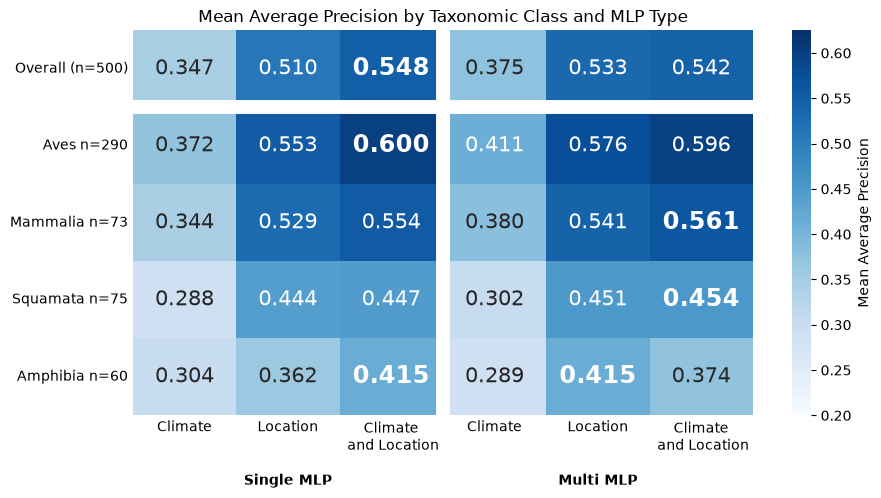
\includegraphics[width=\textwidth]{images/per_class_map_heatmap.png}
    \caption{Heatmap showing MAP for each taxonomic class (excluding crocodylia and testudines) for each MLP input combination. Peak MAP per class is shown bold.}
    \label{fig:mapheatmap}
    \end{subfigure}
    \hfill
    \begin{subfigure}[t]{0.49\textwidth}
    \centering
    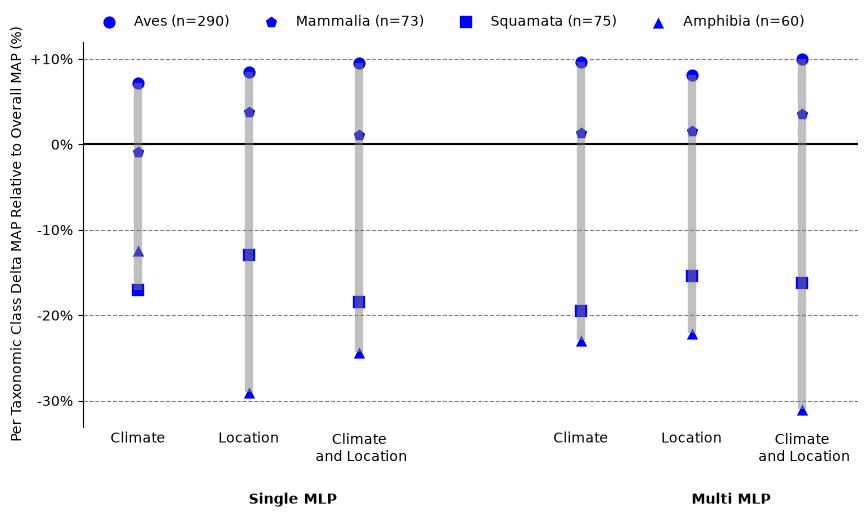
\includegraphics[width=\textwidth]{images/per_class_map_relchange.png}
    \caption{Plot showing the relative deviation (\%) from the model MAP  by taxonomic class (excluding crocodylia and testudines) for each MLP input combination }
    \label{fig:maplines}
    \end{subfigure}
\end{figure}

\section{Conclusion}
We compared a Random Forest, single and multi species MLPs, and seed ensembles of both MLPs for predicting the ranges of 500 species from presence-only data, using location, climate and combined inputs. Both MLPs were able to outperform the RF, and combining location and climate gave the best results for every MLP. The seed ensemble of the single species MLP with combined inputs was the strongest model (test MAP 0.590, against a random baseline of 0.030), and averaging seeds raised MAP slightly for every model and input set.  We applied the models to the projected 2041-2060 climate. With location and climate inputs, about 74\% of current range points, they remain suitable for the climate (sensitivity 0.739), while the model with only the climate diverged more from present ranges (overlap MAP 0.375 against 0.614 \ref{app:fut_ensemble}). The performance of the model varied by taxonomic class, with different models and inputs that performed best for different groups. Therefore, the choice of model may depend on the taxonomic class that we are interested in.  Finally, the resulting future projections cannot be validated yet, because the future ranges have not been observed. Thus, they should not be seen as forecasts where species will occur, but rather as indications about how the suitability of the climate will change for each species.


\bibliography{refs.bib}
\bibliographystyle{plain}

\section*{Statement on Use of Generative AI}

 Generative AI (Claude) was used in formatting the latex document as a text editor. All final text was written by us.
 Several bibtex entries were generated with Google Search AI, though all verified as linked to the intentional papers.
 Academic paper summaries were generated with ELM during the research phase. Though all papers had been independently found and skimmed first. 
 Google Search AI was used for explanation of ecological concepts (e.g. the ecological niche).


\section*{Statement of Contribution}

\begin{center}
  \begin{tabular}{@{}lp{0.5\textwidth}l@{}}
    \toprule
    Student number & Contribution & Proportion (\%) \\
    \midrule
    S2944133 & Worked on: Preprocessing Training \& Test data, Ensemble Method Wrote: Data Preparation, Ensemble Section. (Appendix Data Preparation, Ensemble Method, Future Climate Ensemble) & 25\% \\
    S3028208 & Worked on: Random Forest modelling and experimentation, Result analysis. Wrote: Random Forest section, Data Exploration tuning. (Appendix Decision Tree and Random Forest, data exploration (half)) & 25\% \\
    S1129683 & Worked on: MLP modelling. Results plotting. Wrote: Abstract, intro, MLP section, Results.(Appendix lit review, MLP section) & 25\% \\
    S2237445 & Worked on: Preprocessing historical and future WorldClim data, linked climate data to the training and test. Wrote: Bioclimatic (climate) data, conclusion. (Appendix: data exploration (half), future climate data, limitations) & 25\% \\
    \bottomrule
  \end{tabular}
\end{center}

\appendix

\section*{Appendix}
\renewcommand{\thesubsection}{\Alph{subsection}}

\subsection{Literature Review}\label{lit_rev}

The application of machine learning to species distribution modelling (SDM) begins to appear in academic references in the 1990s \cite{STOCKWELL1992385}. The fundamental principles of an SDM were described by Hutchinson \cite{Hutchinson1957}. Hutchinson introduced the concept of an “ecological niche” in which a species exists if population growth rate remains positive due to the mix of local environmental factors (the niche). Additionally, contrasting species traits allow them to coexist in space whilst occupying a different niche. Model development with machine learning omits ecological hypothesis from the training data and allows the model to discover patterns in the data \cite{GOBEYN2019179}.

Worst case scenario climate change predictions put approximately one third of species globally under threat of extinction \cite{urban2024climate}. The need for species distribution modelling across new environmental and geographic scenarios, known as extrapolation \cite{10.1641/0006-3568}, is increasingly important in resource allocation for species protection. The issue in prediction lies in the fact that future temporal transfers are impossible to validate as the events have not yet occurred \cite{YATES2018790}. Evaluation through alignment with ecological theory \cite{SERRA2026103563}, thorough quantification of uncertainty \cite{lange2025feedforwardfewshotspeciesrange}, and credibility of predictions via explainable AI (XAI) \cite{11345587} are a few established techniques for review of extrapolated SDMs.

Presence-only data, such as the iNaturalist \cite{inaturalist2026} dataset used for this project, where observations record only positive occurrences of species, dominate SDM \cite{https://doi.org/10.1002/ecm.1486}. The generation of absence data is a vital decision in modelling. Miyaji et al \cite{11345587} present a systematic comparison of pseudo-absence strategies. Random sampling was used as the baseline and three further techniques; spatially constrained random sampling, environmentally dissimilar sampling, and a hybrid approach were investigated. The structured strategies significantly improve performance by limiting spatial autocorrelation, especially in tree-based learning models. Their findings motivate the direction of this project.

SDM performance is inconsistent across taxa and regions. Bias towards charismatic and well-studied animals can often appear in community led observation data \cite{lange2025feedforwardfewshotspeciesrange}). To provide inter species links and assess the aforementioned bias, taxonomic data is considered as an addition to the project training set. Data bias also arises from socioeconomic and demographic background. Grade et al. \cite{10.1371/journal.pone.0277223} found that crowdsourced biodiversity datasets often disproportionately represent affluent regions. This contributed to the decision to omit observation density from the training data to focus on species presence rather than abundance.

A wide range of learning methods have been applied to species distribution modelling. \cite{SERRA2026103563} conducted a review of 166 model applications presented in academic literature and found the most widely used model to be maximum entropy (MaxEnt) mentioned in almost 60\%. Followed by random forest (RF) at 12.5\% and third the Neural Network (NN) at 6.3\%, highlighting the dominance of MaxEnt. Maxent is, however, limited to one model per species meaning a loss of inter species or taxa relationships \cite{https://doi.org/10.1111/2041-210x.70262}. RF offers advantages such as the ease with which relative importance of environmental factors can be assessed from the model and the capacity to process a large dataset \cite{https://doi.org/10.1111/j.2006.0906-7590.04596.x}. Neural Networks resistance to overfitting (through regularization flexibility) and a tolerance to errors in training data (common in community led projects) \cite{Worner2014Invasive}. Serra et al. \cite{SERRA2026103563}  advocate an ensemble approach which will be explored in this project.

\subsection{Data Exploration}\label{app:data_exp}

The train dataset is a collection of species observation records from citizen scientists uploaded to iNaturalist. It contains latitude and longitude coordinates for each observation of 500 species. The test dataset has a set of locations for all species in the training set and for each location confirmation of species presence or absence.

Beyond differences between taxonomic groups, Figure~\ref{fig:3} shows how the training observations are distributed among the 500 species. Every species has at least 50 observations, and the counts rise steadily on the logarithmic scale: around 100 observations at rank 120, roughly 220 at the median, and about 1,000 at rank 410. The curve then flattens when it gets to 2,000 for the last 65 species. This indicates that the dataset was capped during preparation, and, as a result, the dataset is unbalanced. This is more prominent when one sees the species with the most  observations that have 40 times more records than the least observed. Moreover, because of the cap, the count of each observation does not reflect how common a species is. This motivates our decision to use binary presence rather than observation counts in the data preparation.

% \begin{figure}[ht]
%     \centering
%     \begin{subfigure}[c]{0.40\textwidth}
%     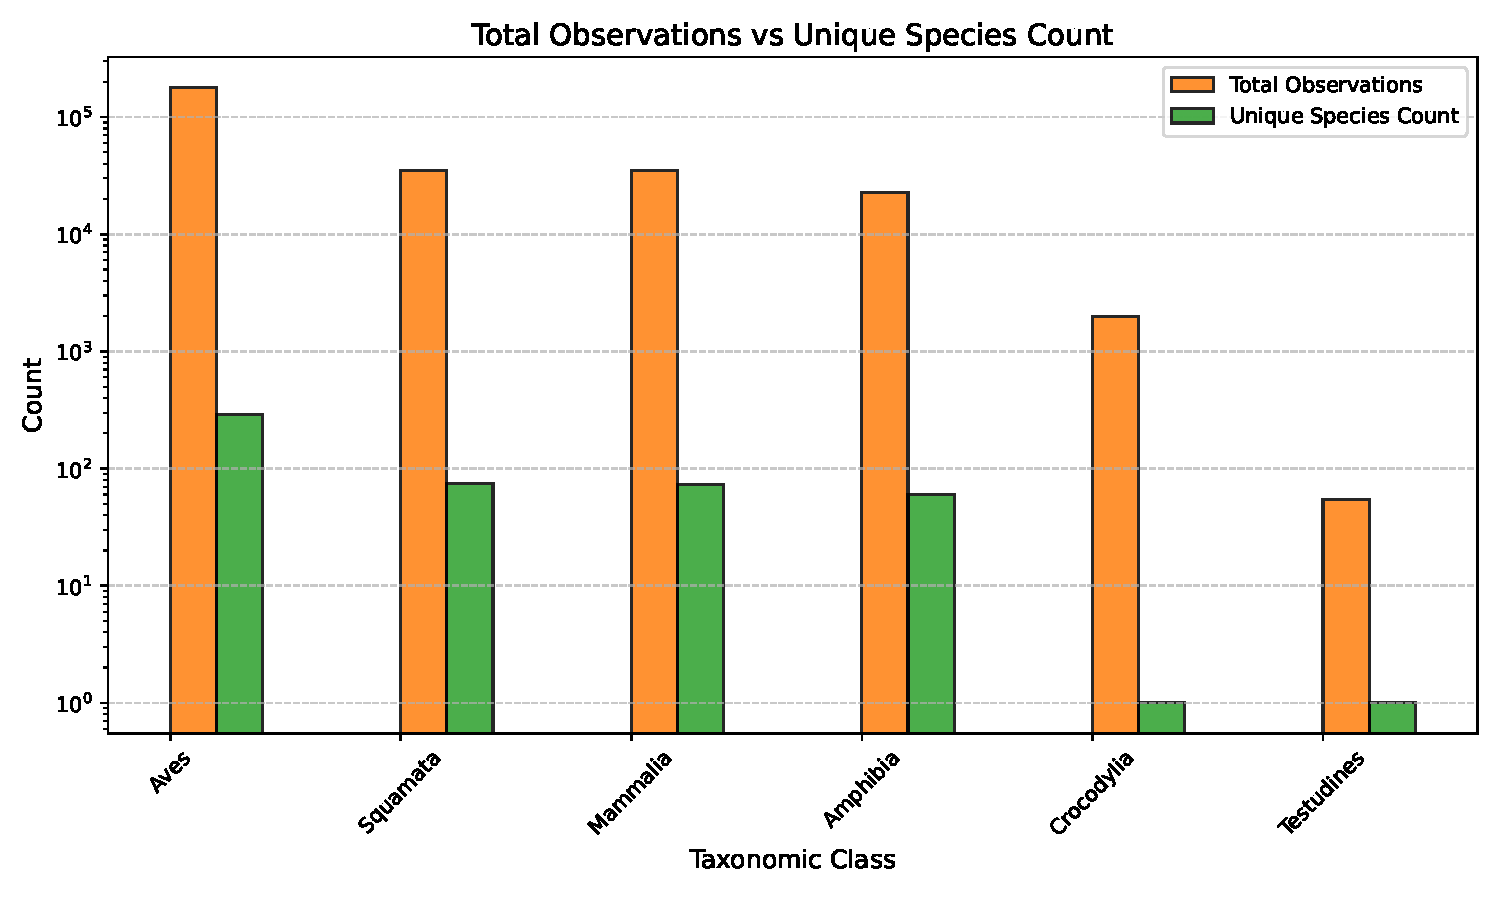
\includegraphics[width=\textwidth]{Data Exploration Graphs/observation_species_count_bar_chart.pdf}
%     \caption{Chart of observation count and unique number of species for each taxonomic class in the dataset with log scale y-axis.}
%     \label{fig:2}
%     \end{subfigure}
%     \hfill
%     \begin{subfigure}[c]{0.40\textwidth}
%     \centering
%     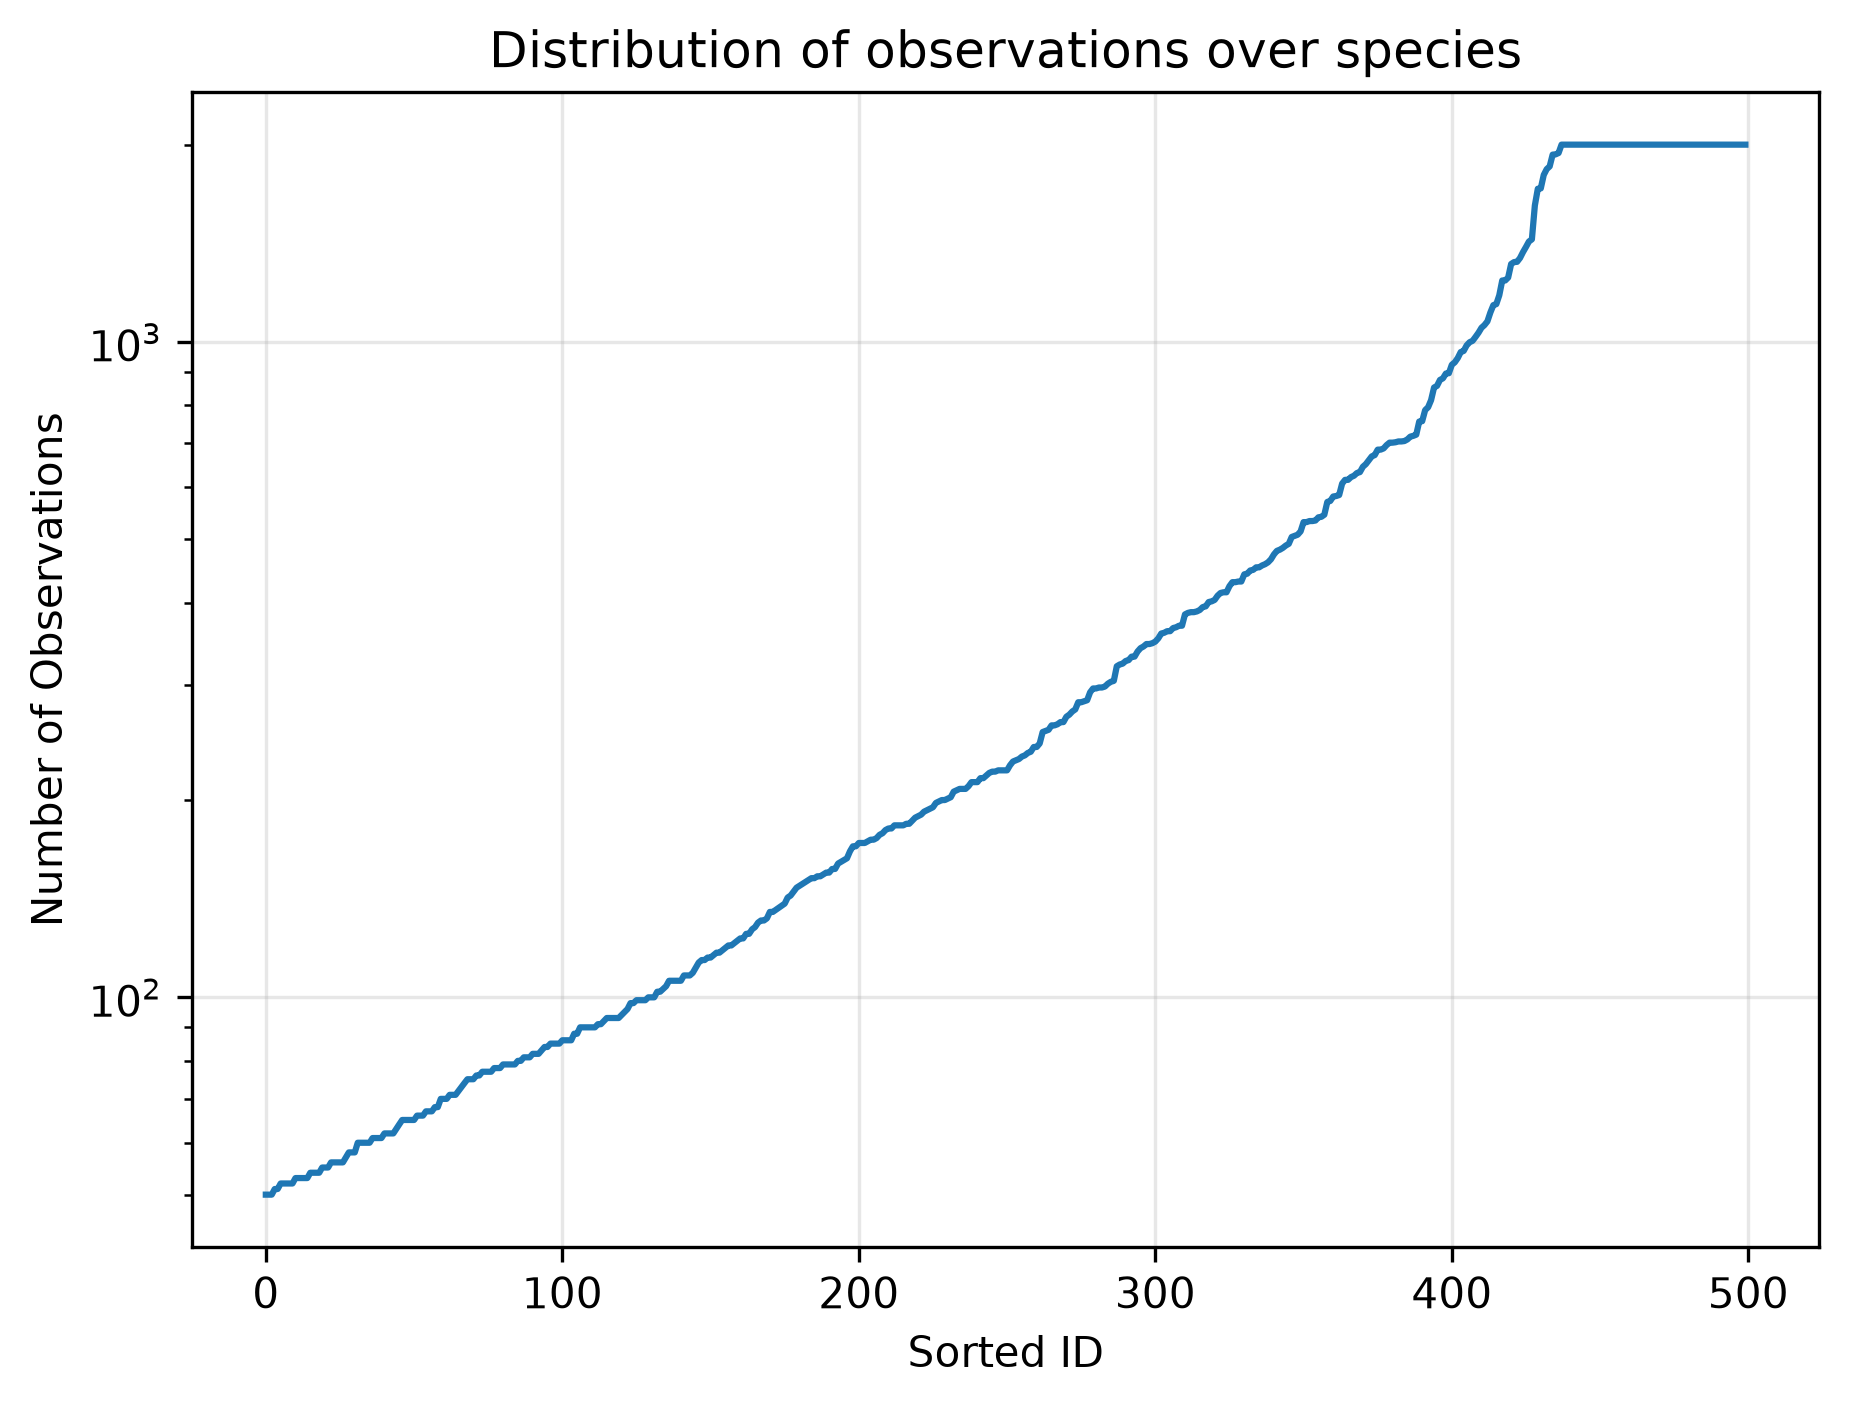
\includegraphics[width=\textwidth]{Data Exploration Graphs/distribution_of_observations.png}
%     \caption{Number of training observations per species, with species sorted  from fewest to most observations. Counts range from 50 to 2000 and the flat section on the right shows that the data were capped at maximum of 2000}
%     \label{fig:3}
%     \end{subfigure}
% \end{figure}

\begin{figure}[H]
    \centering
    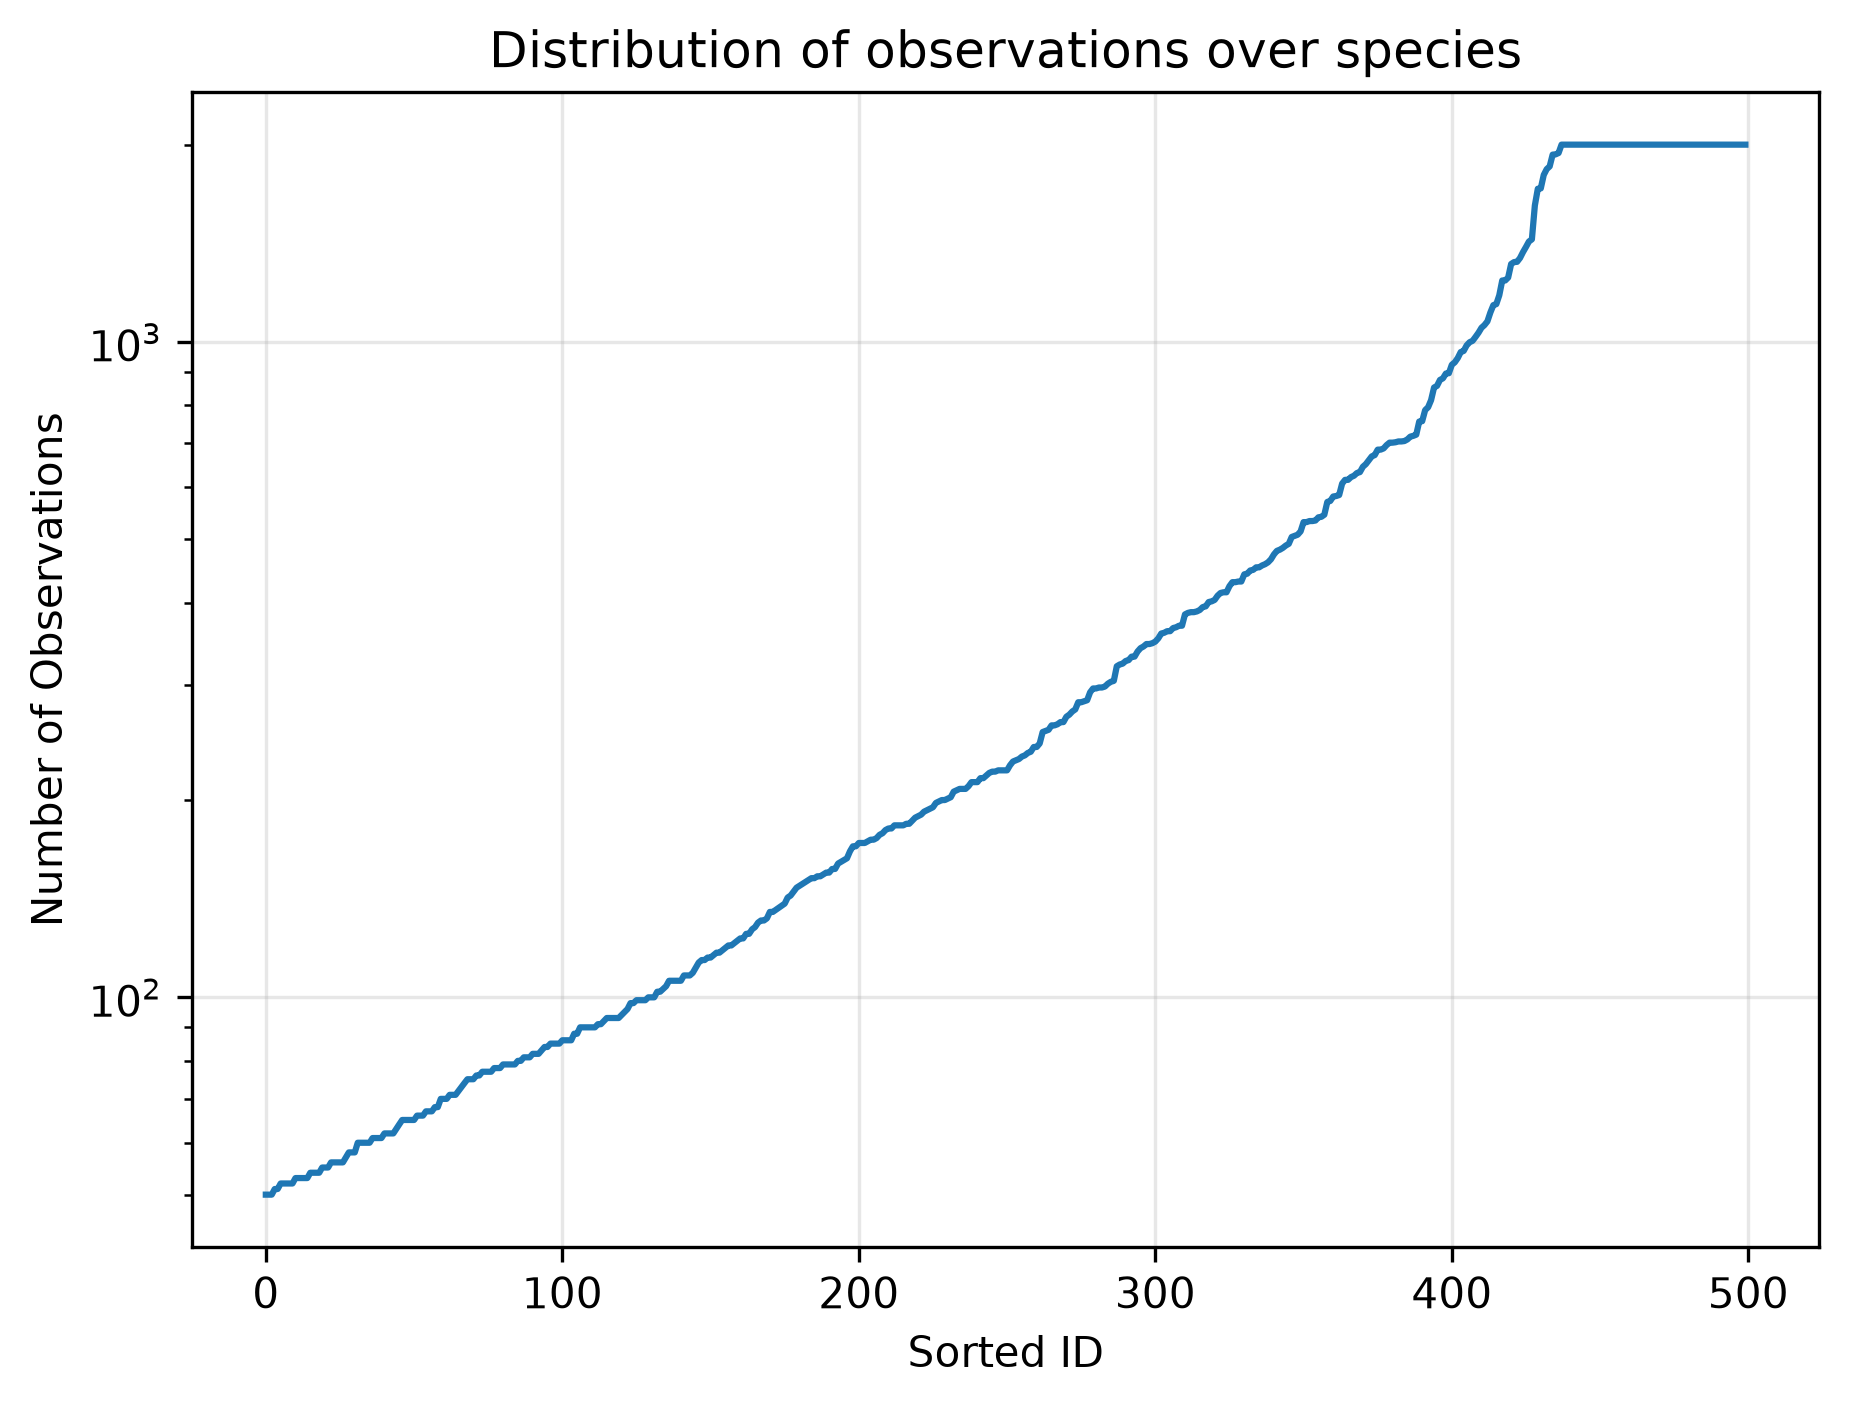
\includegraphics[width=0.3\textwidth]{Data Exploration Graphs/distribution_of_observations.png}
    \caption{Number of training observations per species, with species sorted  from fewest to most observations. Counts range from 50 to 2000 and the flat section on the right shows that the data were capped at maximum of 2000}
    \label{fig:3}
\end{figure}


\subsection{Data Preparation}\label{app:data_prep}
\textbf{Removing ocean sightings:} Sightings more than about 25\,km from land are removed. This removes 798 of the 272,037 sightings (0.3\%). Island and coastal sightings are kept, and no species loses all of its sightings by removing ocean sightings.

\textbf{Spatial binning:} Each species is recorded as present once in a cell, no matter how many times it was observed in that cell, which reduces the 271,239 remaining sightings to 69,497 presences in 16,919 cells. The number of sightings per species per cell ranges from 1 to 700. Binning removes the sighting counts per cell, thins clusters of repeated sightings at popular sites, reducing sampling bias. The counts are kept as $n\_sightings$ for analysis but not used as a model input.

\textbf{Pseudo-absences:} Ocean cells make up about 70\% of the grid, they have no climate data, and would help the model little about where a species is absent on land. A fixed random seed makes the 69,497 pseudo-absences reproducible across single and multi-species training sets. A known limitation we identified is that some pseudo-absences fall inside a species' true but unrecorded range, which is more likely for widespread species. Spatially or environmentally constrained sampling \cite{11345587} is a possible extension. 

\textbf{Training formats:} The per species split was stratified on label and species ID ensuring at least one presence and pseudo absence appeared in each set for train and validation. For model simplicity, the per cell dataset was stratified on number of species present. This preserves the presence-pseudo absence ratio between sets but can lead to rare species (with <5 presences) being assigned wholly to one set. This is highlighted as a limitation of the study and avenue for future study.

\textbf{Taxonomy:} The class is stored as an integer per species and we use it to break down results by group.

\textbf{Test data:} We have not applied any filtering, binning or pseudo-absences to the test file, so it stays fixed for every model. Each point is mapped to its H3 cell to match its climate. For evaluation, we keep only the 89,377 points whose cell has climate data; since the climate grid covers land only, these are the land points. This is done for every input set, including location only, so all models are scored on the same points (Table~\ref{tab:2}).

\textbf{Future climate data:} To project species distributions into the future, we used WorldClim's CMIP6 climate projections for 2041-2060 \cite{fick2017worldclim}. The SSPs (Shared Socioeconomic Pathways) are climate change scenarios up to 2100, used in the IPCC Sixth Assessment Report (2021) \cite{allan2023intergovernmental}. Each one makes different assumptions about things like emissions and population growth, so they estimate different amounts of overall warming. We chose SSP2-4.5, the "middle of the road" scenario, because it is generally seen as the closest to the path the world is currently on. The GCMs are the different global climate models used to make those predictions and they react differently to the same emission. We chose MPI-ESM1-2-HR because its equilibrium climate sensitivity closely matches the IPCC's best estimate: its ECS (long-term warming if CO2 doubles) is 3.0 C \cite{meehl2020context} vs the IPCC's 3 C.

\subsection{Learning Methods}\label{lit_rev_lm}

Each model architecture presented below is evaluated using three distinct input regimes. Location only (using the 4 encoded coordinates), climate only (with the 8 standardised bioclimatic variables) and the combination of the two (12 inputs). The location only establishes a spatial interpolation baseline, climate only has the ability to project to out of spatial range niches, and combining the two allows the model to learn both geographic and environmental suitability.

\subsection{Decision Tree}\label{lit_rev_dt}\textbf{}

An RF has the advantage that by using various decision trees, the resulting classification has an increase in precision and is less prone to over-fitting \cite{JMLR:v12:pedregosa11a}. The use of various decision trees for one model will help have a more precise separation on characteristics between all 500 species and avoid a highly over-fitted model. For the use of this model.

Decision Tree is a supervised model, or one in which the expected labels are known, that is used to make predictions by learning simple decision rules based on the different features\cite{JMLR:v12:pedregosa11a}. In addition, it is one of the few models that has the advantage of being easy to interpret by humans. Our objective in this work is to predict the presence of different species of birds given specific features. Looking at the composition of the data and the objective, we can say with confidence that the use of the Decision Tree model will be of great value. For this model we have the ability to change various parameters. After considering all of them and looking at the hardware at our disposal, we decided to consider \textbf{criterion} and \textbf{max\_depth}. For \textbf{criterion} we have decided to go for ``entropy'' and will look for the optimal \textbf{max\_depth}.

We must define the parameters that will influence the outcome of how the decision trees will observe the characteristics of the data. The \textit{splitting criteria} is the parameter to measure the purity of the the division of a node. We chose between \textit{entropy} or \textit{gini} by looking at the base performance delta between a multi-classification prediction and a binomial one.

\subsection{Decision Tree Training}
We started training some models to have a feel of what we are using and getting to know the tools, their limitations and have a feel for them. We developed a Python notebook that would read the data provided to us, prepare it and fit some Decision Tree models. For the ``X'' data sets where we would find the features that the model will receive, we placed the columns \textbf{``lat''} and \textbf{``lon''} which are passed in their raw format, not transformation, nor adaptation. For the ``y'' data set we would find a list of species that were reported in those locations.

After training the models with different parameters we obtain the results in Table~\ref{tab:dt}.

\begin{table}[ht]
    \centering
    \begin{tabular}{@{}llr@{}}
        \toprule
        Model name & Parameters & Accuracy \\
        \midrule
        Decision Tree T.00 & Default values & 93.65\% \\
        Decision Tree T.01 & criterion=`entropy' & 94.04\% \\
        Decision Tree T.02 & criterion=`entropy', max\_depth=500 & 94.05\% \\
        Decision Tree T.03 & criterion=`entropy', max\_leaf\_nodes=500 & 94.16\% \\
        \bottomrule
    \end{tabular}
    \caption{Table with all trained models and their accuracy reported.}
    \label{tab:dt}
\end{table}

\begin{table}
    \centering
    \begin{tabular}{@{}lr@{}}
        \toprule
        Model name & Accuracy \\
        \midrule
        Random Forest presence & 94.60\% \\
        Random Forest species & 1.73\% \\
        \bottomrule
    \end{tabular}
    \caption{Table with all random forest models and their accuracy.}
    \label{tab:rf_s&p}
\end{table}

\begin{figure}[H]
    \centering
    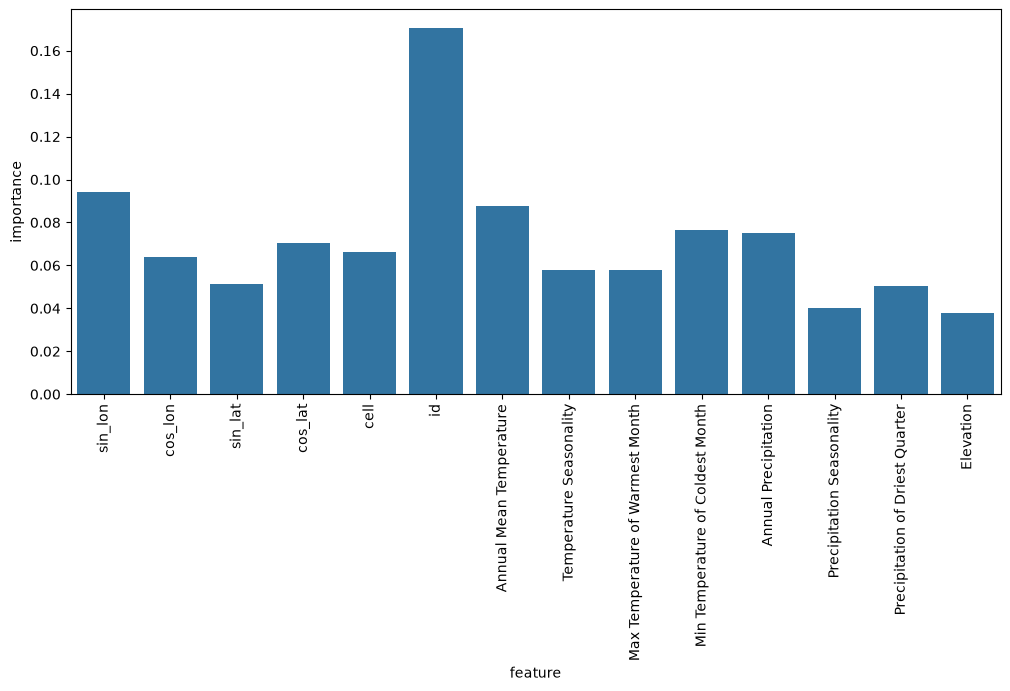
\includegraphics[width=0.75\linewidth]{images/output_features.png}
    \caption{Most used features when training a Random Forest with location, species id \& taxonomy and climate data}
    \label{fig:output_features}
\end{figure}

\begin{figure}[H]
    \centering
    \begin{subfigure}[c]{0.40\textwidth}
    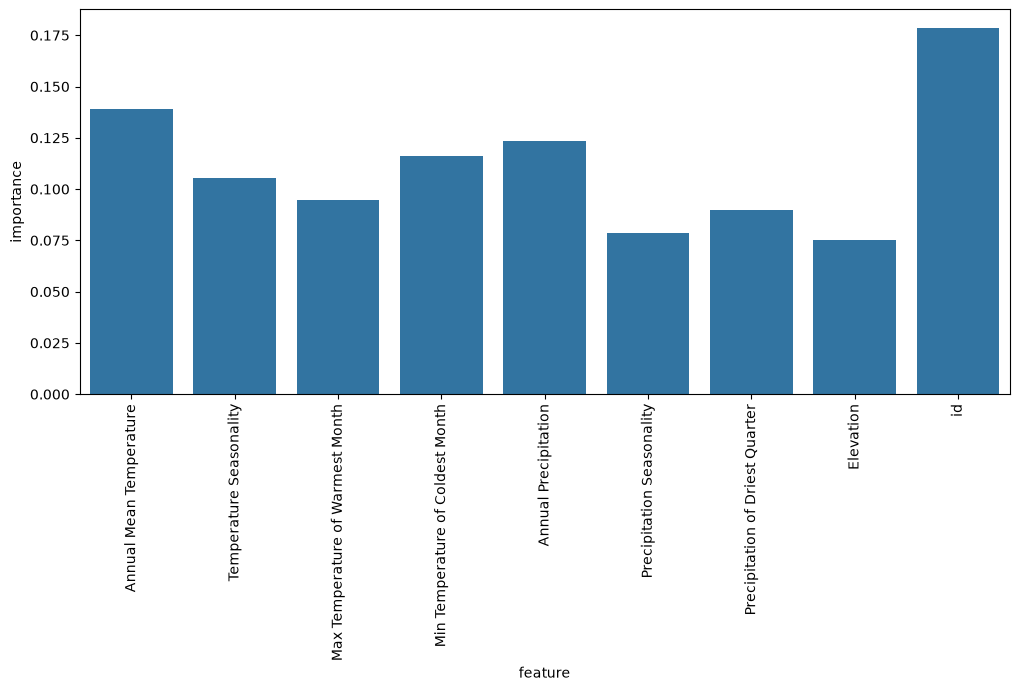
\includegraphics[width=\textwidth]{images/bio_app.png}
    \caption{The features that where given more importance for the Random Forest with only Climate data}
    \label{fig:4}
    \end{subfigure}
    \hfill
    \begin{subfigure}[c]{0.40\textwidth}
    \centering
    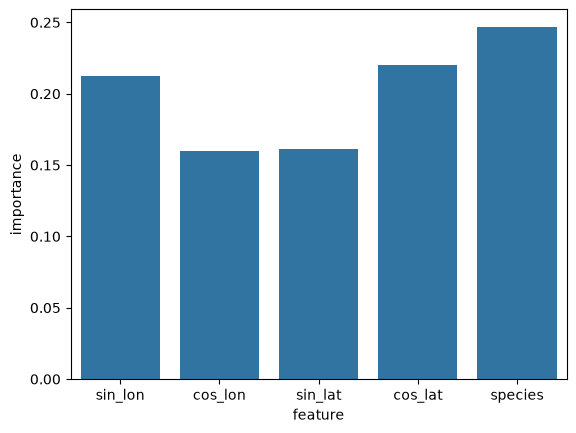
\includegraphics[width=\textwidth]{images/coord_app.png}
    \caption{The features that where given more importance for the Random Forest with location data}
    \label{fig:5}
    \end{subfigure}
\end{figure}

\subsection{Neural Network - Multilayer Perceptron}
\label{appendix:mlp}

A multilayer perceptron (MLP) is a well-documented feedforward artificial neural network. An MLP is capable of handling  complex non-linear problems which can easily be used as a single species or multi species output \cite{https://doi.org/10.1111/2041-210X.14466}. We chose to compare both a single logit/species MLP and a multi logit/species MLP. The multi species model allows shared feature representation across the whole 500 species dataset simultaneously. The single species model learns species interaction by concatenating the inputs with the species indices and passing it to the embedding layer. The embedding layer is a learned parameter which prevents arbitrary ordinal relationships developing due to the species indices \cite{google_ml_embeddings}. It was preferred to one-hot-encoding as many of the input locations contain only a single presence. A 500 dimensional vector \(o_i\), with 499 zeros, leaving only row \(i\) active in the first layer weight matrix \(o_i^TW=W[i,:]\), isolating species from one another.
\\\\
For definition of network capacity and regularisation the climate plus location inputs were judged to be the most applicable to future projections, and therefore used for hyperparameter tuning and carried forward across experiments. A short ablation was conducted for both MLPs, targeting reduced generalisation gap and maximised MAP on the validation set. For the multi species MLP a binary mask was applied to the loss calculation (equation ~\ref{eq:masked_bce}) to prevent the network overfitting on the 32 million background absences that were not generated as pseudo absences. This allowed the model to maintain the 0.5 prior of presence to pseudo absence for each species.
\\\begin{equation}
    \mathcal{L}_{\text{masked}} = \frac{\sum_{i,j} M_{ij} \, \ell_{\text{BCE}}(z_{ij}, y_{ij})}{\sum_{i,j} M_{ij}}
    \label{eq:masked_bce}
\end{equation}
It was found that dropout (p = 0.15) combined with AdamW weight decay (1e-4 single, 3e-4 multi) reduced generalisation gap, alongside no loss in training accuracy, indicating the unregularised network was overfitting to the training data. The remaining fixed network capacity and hyperparameters are shown in Table~\ref{tab:nn_arch} and \ref{tab:nn_hyperparams}. Early stopping was implemented at peak MAP for each different training input.


\begin{table}[ht]
    \centering
    \small
    \setlength{\tabcolsep}{4pt}
    \begin{tabularx}{\linewidth}{@{} l >{\raggedright\arraybackslash}X l >{\raggedright\arraybackslash}X @{}}
        \toprule
        Model & Layers (nodes) & Activation & Loss \\
        \midrule
        Single Logit & Input $(N + \text{sp}_i) \rightarrow \text{Embedding } (32) \rightarrow \text{Linear} \times 3\ (128) \rightarrow \text{Raw logit } (1)$ & ReLU & BCE with Logits Loss \\
        \addlinespace[3pt]
        Multi Logit & Input $(N) \rightarrow \text{Linear} \times 3\ (128) \rightarrow (500)$ & ReLU & Masked BCE with Logits Loss \\
        \bottomrule
    \end{tabularx}
    \caption{Neural network architectures across input feature sets ($N \in \{4, 8, 12\}$) for species $\text{sp}_i$. The 128-node layers are linear with ReLU activation, outputting raw logits. The 32-node layer is the species embedding matrix.}
    \label{tab:nn_arch}
\end{table}

\begin{table}[ht]
    \centering
    \small
    \begin{tabular*}{\linewidth}{@{\extracolsep{\fill}} lllrrrr @{}}
        \toprule
        & \multicolumn{2}{c}{Regularisation} & & \multicolumn{3}{c}{Epochs} \\
        \cmidrule(lr){2-3} \cmidrule(l){5-7}
        Model & Dropout & Weight Decay & Learning Rate & 4 input & 8 input & 12 input \\
        \midrule
        Single Logit & $p = 0.15$ & $1.0 \times 10^{-4}$ & $5.0 \times 10^{-3}$ & 21 & 38 & 22 \\
        Multi Logit & $p = 0.15$ & $3.0 \times 10^{-4}$ & $5.0 \times 10^{-3}$ & 27 & 22 & 11 \\
        \bottomrule
    \end{tabular*}
    \caption{Training hyperparameters and early-stopping epochs across input feature sets ($N \in \{4, 8, 12\}$) for the single-logit and multi-logit neural network architectures.}
    \label{tab:nn_hyperparams}
\end{table}
\subsection{MLP - Training Curves}
Training curve example for Single Species, 8 input (climate), MLP. Regularisation was tuned to minimise the gap between validation and training accuracy. Early stopping criteria (for a subsequent run) was selected from the peak in MAP.
\begin{figure}[H]
    \centering
    \begin{subfigure}[c]{0.450\textwidth}
    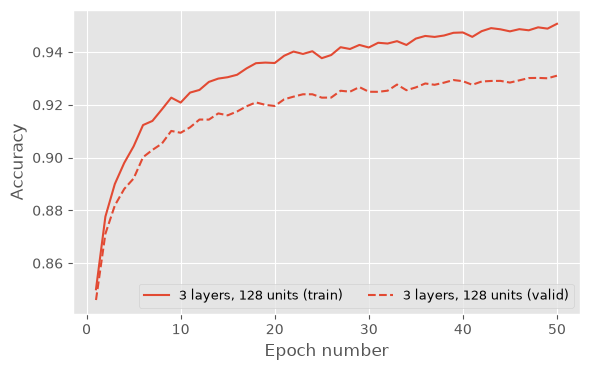
\includegraphics[width=\textwidth]{images/learningcurve_acc.png}
    \caption{50 Epoch trace of training vs validation accuracy for the Single Species, 8 input (climate), MLP }
    \label{fig:lcacc}
    \end{subfigure}
    \hfill
    \begin{subfigure}[c]{0.450\textwidth}
    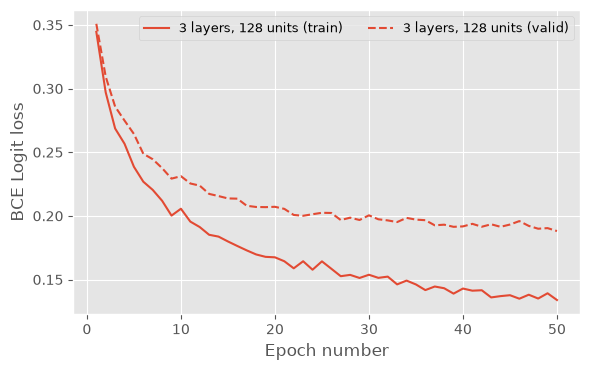
\includegraphics[width=\textwidth]{images/learningcurve_bce.png}
    \caption{50 Epoch trace of training vs validation BCE for the Single Species, 8 input (climate), MLP }
    \label{fig:lcbce}
    \end{subfigure}
\end{figure}

\begin{figure}[ht]
    \centering
    \begin{subfigure}[c]{0.450\textwidth}
    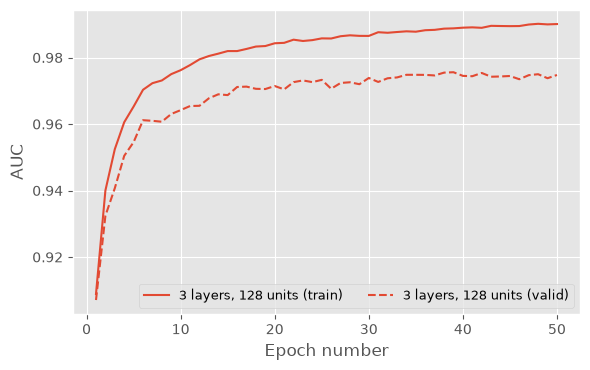
\includegraphics[width=\textwidth]{images/learningcurve_auc.png}
    \caption{50 Epoch trace of training vs validation AUC for the Single Species, 8 input (climate), MLP }
    \label{fig:lcauc}
    \end{subfigure}
    \hfill
    \begin{subfigure}[c]{0.450\textwidth}
    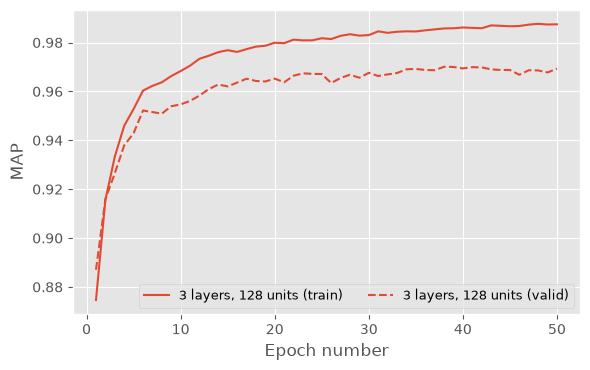
\includegraphics[width=\textwidth]{images/learningcurve_map.png}
    \caption{50 Epoch trace of training vs validation MAP for the Single Species, 8 input (climate), MLP }
    \label{fig:lcmap}
    \end{subfigure}
\end{figure}

\subsection{Ensemble Method}\label{app:ensemble}

\textbf{Method:} Training a neural network on fixed data has three sources of randomness: the initial weights, the dropout masks and the order of the training batches. Each member of the ensemble is the same network, it is trained with the same data and train/val split, but with different model seeds that control only these three sources of randomness. Because of this, the members agree and disagree on the data. By averaging the predicted probabilities of the independently initialised networks we can reduce the variance.

For each MLP and input set, the three members are trained with hyper-parameters and early-stopping epochs in Table~\ref{tab:nn_hyperparams}. All members are given equal weights as they share the same architecture and data. The presence threshold for each species is chosen on the validation set, this is done to maximise the TSS, using the averaged validation probabilities, so ensemble is thresholded similar to the single models. Each of the members is also evaluated on the same 89,377 land test points.

\begin{table}[ht]
    \centering
    \small
    \renewcommand{\arraystretch}{0.92}
    \setlength{\aboverulesep}{2pt}
    \setlength{\belowrulesep}{2pt}
    \setlength{\tabcolsep}{2pt}
    \newcommand{\hdr}[1]{\begin{tabular}[b]{@{}r@{}}#1\end{tabular}}
    \begin{tabular*}{\linewidth}{@{\extracolsep{\fill}} llrrrrrr @{}}
        \toprule
        Model & Member & \hdr{Val. \\ MAP} & \hdr{Test \\ MAP} & \hdr{Test Macro \\ TSS} & \hdr{Test Macro \\ AUC} & \hdr{Test \\ Sensitivity} & \hdr{Test \\ Specificity} \\
        \midrule
        \multirow{4}{*}{Single MLP}
            & Seed 0   & 0.980 & 0.526 & 0.738 & 0.986 & 0.757 & 0.981 \\
            & Seed 1   & 0.982 & 0.524 & 0.748 & 0.986 & 0.768 & 0.980 \\
            & Seed 2   & 0.982 & 0.532 & 0.739 & 0.986 & 0.758 & 0.981 \\
            & Ensemble & 0.984 & 0.590 & 0.746 & 0.989 & 0.762 & 0.985 \\
        \midrule
        \multirow{4}{*}{Multi MLP}
            & Seed 0   & 0.981 & 0.539 & 0.743 & 0.986 & 0.768 & 0.975 \\
            & Seed 1   & 0.982 & 0.530 & 0.759 & 0.985 & 0.783 & 0.975 \\
            & Seed 2   & 0.979 & 0.537 & 0.766 & 0.985 & 0.791 & 0.974 \\
            & Ensemble & 0.983 & 0.559 & 0.754 & 0.987 & 0.777 & 0.977 \\
        \bottomrule
    \end{tabular*}
    \caption{Seed ensemble of each MLP with location and climate inputs (12 inputs), on land test points. Metrics are macro averages over species.}
    \label{tab:seed_ens}
\end{table}

\textbf{Results:} Table~\ref{tab:seed_ens} compares the three seeds of each MLP with their ensemble, using location and climate inputs. Averaging the three seeds raised the test MAP by 0.062 for the single species MLP (from a mean of 0.527 to 0.590) and by 0.023 for the multi species MLP (from 0.535 to 0.559), and in both cases the ensemble was able to outperform every individual seed. The individual seeds ranged from 0.524 to 0.532 test MAP for the single species MLP and from 0.530 to 0.539 for the multi species MLP.

This gain over individual seeds is in metrics not dependent on threshold. Test MAP and AUC improved, but TSS stayed within the range of the member seeds, with slightly higher and slightly lower, specificity and sensitivity respectively. This is likely because averaging improves how the predictions are ranking the locations, whereas the TSS which depends on threshold, which itself is chosen on validation data built partly on the pseudo-absences.

\subsection{Future Climate Ensemble}\label{app:fut_ensemble}
\textbf{Method:} The single species MLP seed ensemble is applied to the 2041-2060 SSP2-4.5, MPI-ESM1-2-HR climate. Everything is kept identical to the current-climate runs (Table~\ref{tab:nn_hyperparams}), and the validation MAP and per-species TSS thresholds are also unchanged. Only the climate inputs of the test points are changed with the future climate values, normalised with the historical means and standard deviations. Predictions are compared against today's IUCN ranges on the land test points. Since future species ranges are not known, the metrics measure how much the predicted future ranges agree with the present range rather than how accurate it is. 

\begin{table}[ht]
    \centering
    \small
    \renewcommand{\arraystretch}{0.92}
    \setlength{\aboverulesep}{2pt}
    \setlength{\belowrulesep}{2pt}
    \setlength{\tabcolsep}{2pt}
    \newcommand{\hdr}[1]{\begin{tabular}[b]{@{}r@{}}#1\end{tabular}}
    \begin{tabular*}{\linewidth}{@{\extracolsep{\fill}} llrrrrrr @{}}
        \toprule
        Inputs & Member & \hdr{Val. \\ MAP} & \hdr{Overlap \\ MAP} & \hdr{Overlap Macro \\ TSS} & \hdr{Overlap Macro \\ AUC} & \hdr{Overlap \\ Sensitivity} & \hdr{Overlap \\ Specificity} \\
        \midrule
        \multirow{4}{*}{Loc + Clim}
            & Seed 0   & 0.980 & 0.546 & 0.716 & 0.986 & 0.734 & 0.982 \\
            & Seed 1   & 0.982 & 0.549 & 0.731 & 0.986 & 0.749 & 0.982 \\
            & Seed 2   & 0.982 & 0.554 & 0.714 & 0.987 & 0.733 & 0.982 \\
            & Ensemble & 0.984 & 0.614 & 0.725 & 0.989 & 0.739 & 0.986 \\
        \midrule
        \multirow{4}{*}{Climate}
            & Seed 0   & 0.968 & 0.327 & 0.634 & 0.956 & 0.687 & 0.946 \\
            & Seed 1   & 0.969 & 0.310 & 0.623 & 0.954 & 0.679 & 0.944 \\
            & Seed 2   & 0.969 & 0.324 & 0.622 & 0.957 & 0.673 & 0.949 \\
            & Ensemble & 0.975 & 0.375 & 0.624 & 0.961 & 0.669 & 0.955 \\
        \bottomrule
    \end{tabular*}
    \caption{Single species MLP seed ensemble applied to the 2041--2060 SSP2-4.5 climate. Overlap metrics compare future predictions with today's IUCN ranges on land test points, and are macro averages over species. They measure agreement with the present range, not accuracy.}
    \label{tab:future}
\end{table}

\textbf{Results:} Table~\ref{tab:future} shows that, as in the current climate conditions, the seed ensemble was able to raise overlap MAP over every member seed: by 0.064 for location and climate inputs (from a seed mean of 0.550 to 0.614) and by 0.055 for climate only inputs (from 0.320 to 0.375). AUC also increased, while TSS stayed within the range of the seeds, matching the current-climate behaviour (Appendix~\ref{app:ensemble}). With location and climate inputs, about 74\% of the current IUCN points are predicted to remain suitable for 2041-2060 measured by sensitivity (0.739), and very few points are outside range as present measured by specificity (0.986). The climate only model agrees less with present ranges. The predictions follow shift in suitable climate rather than in species' current range as it is not bounded geographically.

\begin{figure}[ht]
    \centering
    \begin{subfigure}[c]{0.490\textwidth}
    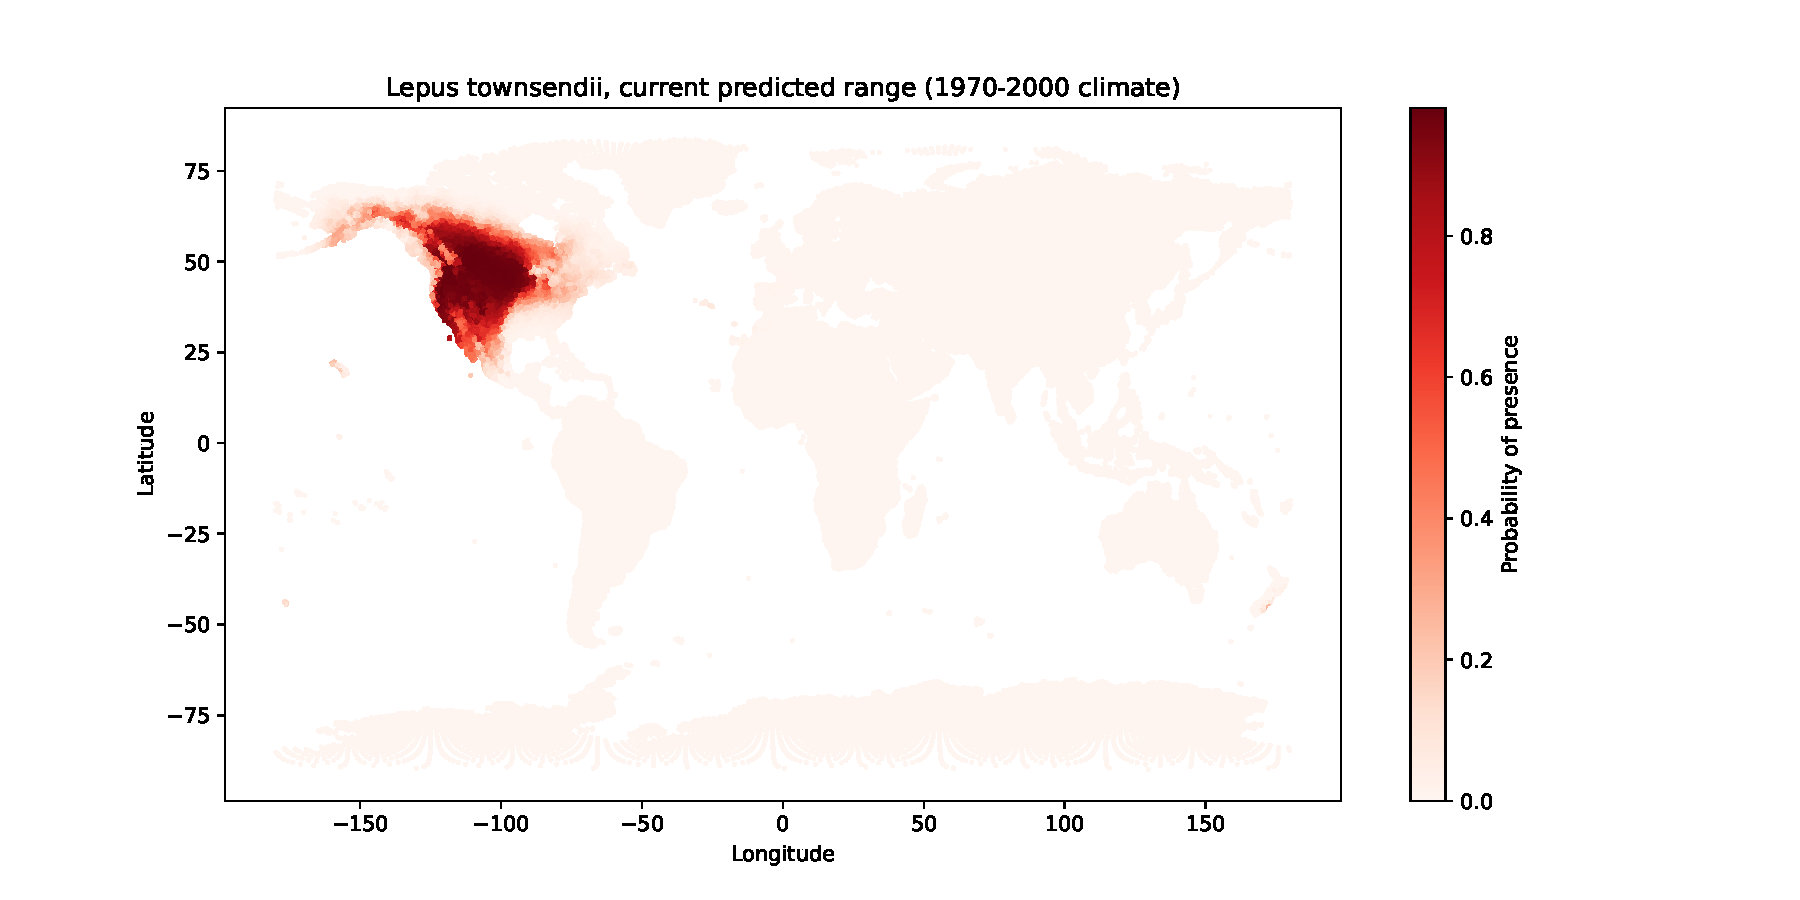
\includegraphics[width=\textwidth]{images/current.pdf}
    \caption{Current climate (1970-2000). }
    \label{fig:range_current}
    \end{subfigure}
    \hfill
    \begin{subfigure}[c]{0.490\textwidth}
    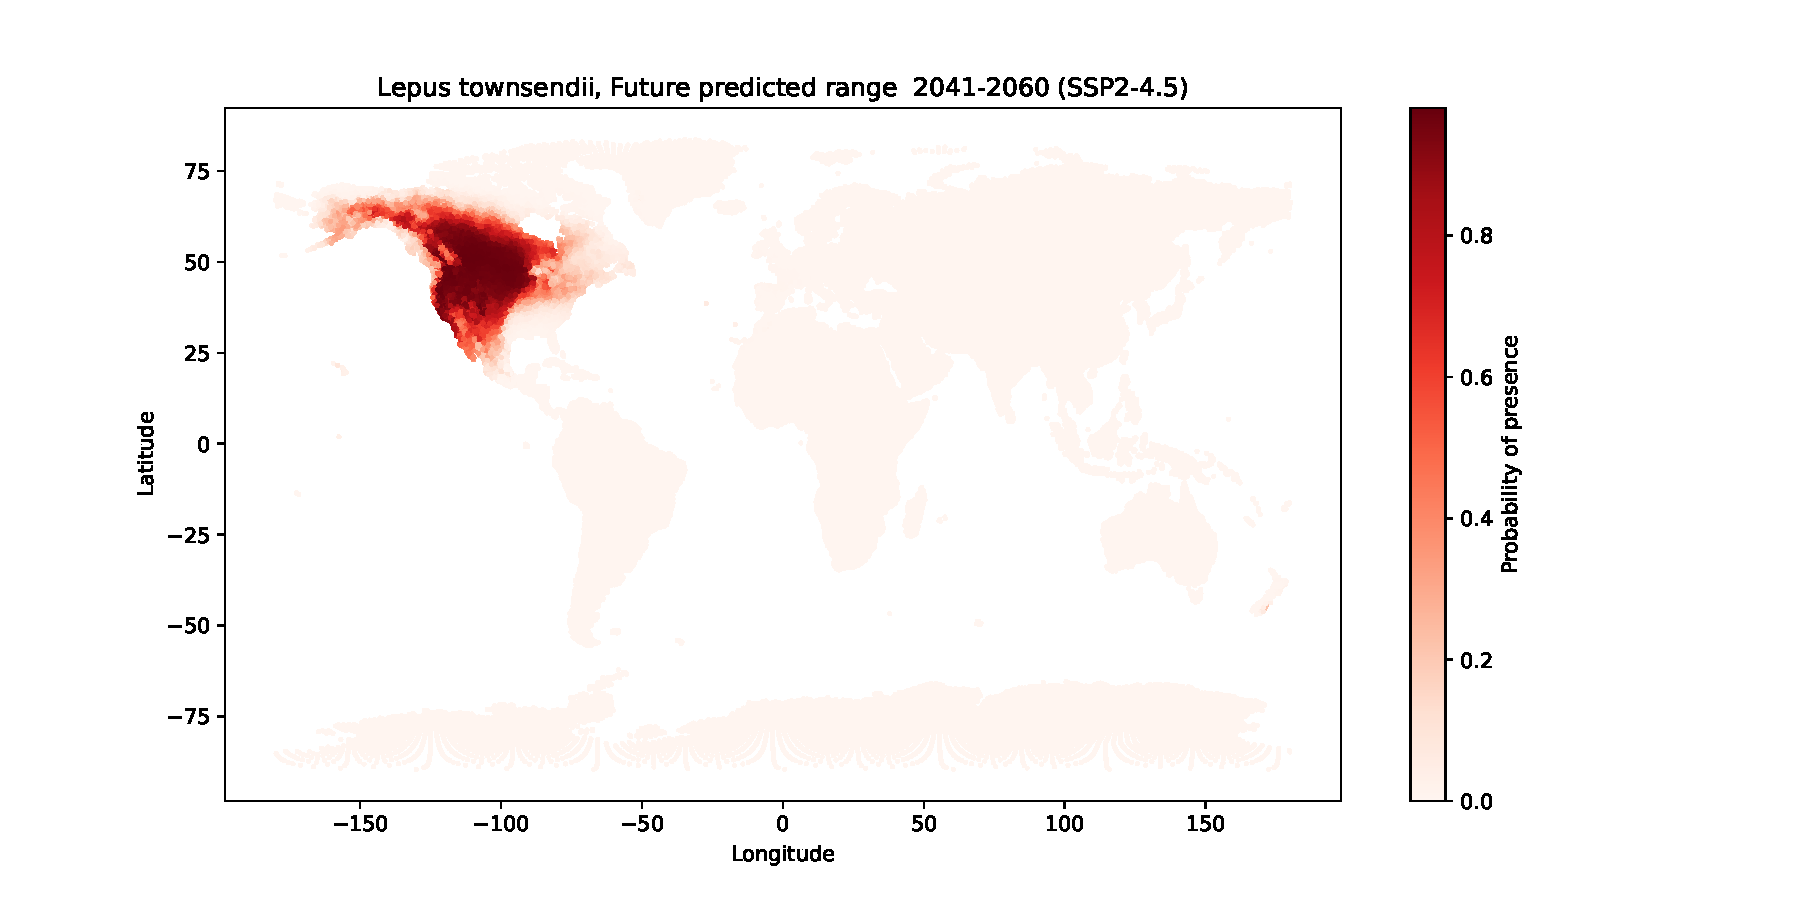
\includegraphics[width=\textwidth]{images/future.pdf}
    \caption{Future climate (2041-2060, SSP2-4.5).}
    \label{fig:range_future}
    \end{subfigure}
    \caption{Predicted range of \textit{Lepus townsendii} (White-tailed jackrabbit) from the single species MLP ensemble with location and climate inputs.}
\end{figure}

\subsection{Additional Results}\label{add_res}

\begin{figure}[H]
    \centering
    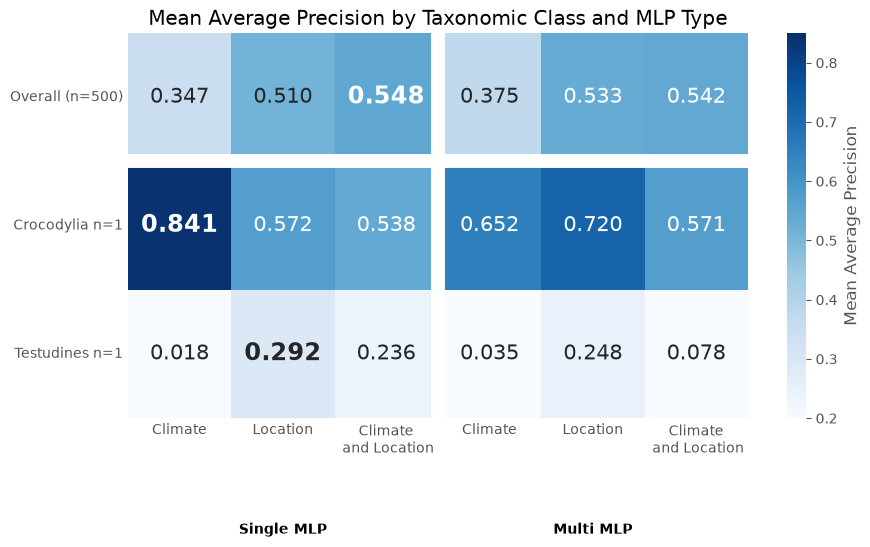
\includegraphics[width=0.75\linewidth]{images/cror_turt_map_heatmap.png}
    \caption{Heatmap showing mean average precision for crocodylia and testudines for each MLP and input combination. Peak MAP for each class is highlighted with bold font.}
    \label{fig:heatmap}
\end{figure}

\subsection{Evaluation Metrics}\label{eval_metric}

We use \textbf{Mean average precision (MAP)} as our primary evaluation metric. It takes the unweighted mean of Average Precision (AP) across all 500 species so rare species carry equal weight to common ones. It needs no threshold, and a random model scores a MAP of 0.030 on land, which gives a clear baseline. It is also a commonly used SDM metric in the literature \cite{cole2023sinr, lange2025feedforwardfewshotspeciesrange}. To expose disparities in the data hidden by the overall mean we inspect MAP by taxonomic class (\(\frac{1}{N_{c}}\sum_{i \in c} \text{AP}_i\)). \textbf{ROC-AUC} is reported for consistency with the literature \cite{SERRA2026103563}, but is excluded from model selection decisions. ROC-AUC is invariant to class prevalence, and since AUC integrates true positive rate across the entire false positive rate range, AUC is close to 1 for almost any model (evidenced in the MLP results presented in Table \ref{tab:2}, ranging from 0.957-0.989). True absences are easily predicted in the ocean or other continents\cite{11345587}.\textbf{True Skill Statistic} (\(TSS = sensitivity + specificity - 1\)) scores binary range maps, which are needed to measure how much of a range persists. Like ROC-AUC it is invariant to prevalence \cite{allouche2006tss}. To avoid leakage from the test set, we maximise TSS per species for each model against the validation set and freeze them for application to the test set.

\subsection{Limitations}
The training data reflect the sampling biases of observations from the community, and small classes such as Crocodylia and Testudines contain only a few species for us to make good conclusions. For future projections, we only used a single climate model (GCM: MPI-ESM1-2-HR), scenario (SSP2-4.5) and period (2041-2060). Therefore, climate model and scenario uncertainty are not captured and the models describe climatic suitability only.
Furthermore, the train validation split for the multi models is stratified by how many species are in a cell, not by each species. So there is a chance a species with low range or observations can land all in one set (all in train or all in validation). If they are all in validation, the model never sees them during training, and if they are all in training, they cannot be assessed or tuned on the validation set. Moreover, pseudo absences are random and sometimes can be generated close to the actual species ranges, creating noisy data. Another limitation is that some of the selected bioclimatic variables are likely to be affected by multicollinearity, which can make the models less reliable. Lastly, the classes are unbalanced, with Aves making up 290 of the 500 species. So, overall metrics are dominated by birds and may not reflect performance of other groups.

\end{document}

%%% Local Variables:
%%% mode: latex
%%% TeX-master: t
%%% End:
